\documentclass[20pt]{article}
\usepackage[utf8]{inputenc}
\usepackage{amsmath}
\usepackage{amssymb}
\usepackage{amsfonts}		 
\usepackage{enumitem}
\usepackage{fancyheadings}
\usepackage{mathtools}
\usepackage{tikz}
\usepackage{fancybox}
\usetikzlibrary{automata,positioning}
\DeclarePairedDelimiter{\ceil}{\lceil}{\rceil}
\DeclarePairedDelimiter\floor{\lfloor}{\rfloor}
\usepackage[margin=3cm]{geometry}
\usepackage{changepage}

\title{CSC263H1 Homework 1}
\author{Tony Yang, Wendy Guo, Martin Chak}
\date{January 16th 2020}

\begin{document}

%BEGIN TITLE PAGE

\maketitle
\noindent
\textbf{Question 1:}\\
\begin{text}
    Done by: Tony Yang\\
    Written by: Martin Chak\\
\end{text}

\noindent
\textbf{Question 2:}\\
\begin{text}
    Done by: Tony Yang, Martin Chak, and Wendy Guo\\
    Written by: Martin Chak and Wendy Guo\\
\end{text}

%END TITLE PAGE

\newpage

%BEGIN Q1
\section*{Question 1}
\textbf{Done by: Wentao Yang; Written by: Martin Chak}\\
\noindent
\begin{text}
    \indent The function $NOTHING(A)$ has an input array $A [1...n]$ (This means $A$'s indices range from $1$ to $n$) with $n \geq 2$. Assuming assignment, comparison, and arithmetic operations take constant time. Let $T(n)$ be the worst-case time complexity of calling $NOTHING(A)$ on an $A$ of size $n \geq 2$. Give a tight asymptotic bound for $T(n)$ so that there is a function $f(n)$ such that $T(n)$ is $\Theta(f(n))$. We pick $f(n) = n$ and show $T(n)$ is $\Omega(n)$ and $T(n)$ is $O(n)$.\\
\end{text}

\noindent
\underline{\textbf{Worst Case Lower Bound}}\\
\begin{text}
    \indent Let us first show $T(n)$ is $\Omega(n)$. Let $n \in \mathbb{N}$ s.t. $n \geq 2$. We then let $A$ be a list of integers where index 1 is $n$ and the value of each successive index is one less such that $A = [n, n - 1,...,1]$. We must show that the function has at least $n$ steps.\\
    \noindent
    \indent When we execute the function, line 1 assigns $n = A.size$ which has $n$ elements, taking the first step. Then we enter the outer for-loop on line 2 and begin iterating on the inner for-loop on line 3. The if-statement on line 4 will never execute, since $A[n-j+1] = j$ as we defined $A[1] = n$, $A[2] = n-1$, etc. Once the inner for-loop has terminated after at least $n$ steps/iterations of the loop, we reach line 5. While $i = 1$, as we are on the first iteration of the for-loop, the first if-condition: $A[i] \neq n-i$ holds since $A[1] \neq n-1$ as a consequence of $A$'s definition that $A[1]=n$ and the assumption that $n \geq 2$ holds. The function then terminates pre-maturely on line 5 and returns, ending the function after a total of $n + 2$ steps.Therefore the worst-case function $T(n)$ takes at least $n$ steps and it is $\Omega(n)$.\\
\end{text}

\noindent
\underline{\textbf{Worst Case Upper Bound}}\\
\begin{text}
    \indent Let us now show $T(n)$ is $O(n)$. Let $n \in \mathbb{N}$ s.t. $n \geq 2$. We let $A$ be an arbitrary list of integers such that the length of $A$ is $n$. We must show that the function takes at most $n$ steps.\\
    \noindent
    \indent When we execute the function, line 1 assigns $n=A.size$, taking the first step. Like before, we enter the outer for-loop, but once we reach the inner for-loop we reach our first possible termination statement on line 4. We then split up the proof into two cases, one where the program terminates early on line 4, and one where the program terminates later on other lines.\\
\end{text}

\noindent
\textbf{Case 1: Line 4 Does Not Return}\\
\begin{text}
    \indent For this to hold, the condition $A[n-j+1] \neq j$ must never hold for any $j \in [1,n]$. The only input $A$ that allows this is where $A$ is a list of descending numbers from $n$ to $1$, such that $A = [n, n-1, ..., 2, 1]$.\\
    \noindent
    \indent After the first assignment step, we reach the first iteration of the outer for-loop, the inner for-loop will get to iterate $n$ times since $A[n-j+1] = j$ for all $j \in [1,n]$. After the inner for-loop finishes, line 5 will check if $A[i] \neq n - i$, which holds since $i = 1$ on this iteration, and $A[1] = n \neq n-1$. Line 5 then takes $1$ step to return and then the program finishes with a total of $n+2$ steps\\
\end{text}

\noindent
\textbf{Case 2: Line 4 Returns}\\
\begin{text}
    \indent For this to hold, the condition $A[n-j+1] \neq j$ must hold during an iteration of the inner for-loop. This case covers all other inputs $A$ where $A[n-j+1] \neq j$ for $j \in [1,n]$.\\
    \noindent
    \indent On the first iteration of the outer for-loop, line 4 will execute on the $j-ith$ iteration of the inner for-loop, where the condition first holds at $j$. At most the inner for-loop can iterate $n-1$ times before the condition holds, terminating the function with a final step, leaving a total of $n+1$ steps. Therefore for any input list $A$ of size $n$, the program will take at most a total of $n+2$ steps to terminate, showing that the worst case function $T(n)$ is $O(n)$.\\
\end{text}


\noindent
\begin{text}
    We have then shown that $T(n)$ is both $\Omega(n)$ and $O(n)$, this implies that $T(n)$ is $\Theta(n)$ as required
    
    \hfill$\blacksquare$
\end{text}
%END Q1

\newpage

%BEGIN Q2
\section*{Question 2}
\textbf{Done by: Wentao Yang, Wendy Guo and Martin Chak; Written by: Martin Chak and Wendy Guo}
\begin{text}
Let $I_n$ be a set of $n$ integers $\{1, 2, ..., n\}$ where $n$ is some power of 2. We want to define a data structure so that the following operations are supported for a set $S \subseteq I_n$:
\end{text}
\begin{align}
    INSERT(j) &: \text{insert integer $j$ into $S$}\nonumber\\
    DELETE(j) &: \text{delete integer $j$ from $S$}\nonumber\\
    MEMBER(j) &: \text{return \textbf{true} if $j \in S$, otherwise return \textbf{false}}\nonumber\\
    MAXIMUM &: \text{return the greatest integer in $S$}\nonumber
\end{align}

\noindent
\begin{text}
    We then need to support the above operations while keeping the worst-case time complexity of operations $INSERT(j)$, $DELETE(j)$, and $MAXIMUM$ to be $O(log(n))$. While the worst-case time complexity of $MEMBER(j)$ is $O(1)$. We also need to make sure that the data structure takes only $O(n)$ bits of storage.\\
    
    \noindent
    So we create a data structure using an $n$-bit vector and a complete binary search tree. Where $n$ is the $k$-th power of 2 such that $k = log_{2}(n)$. Each node stores a single bit representing 0 or 1, and the $k$-th level of nodes represent an $n$-bit vector for the elements of $S$. In any case we will always have exactly $2n-1$ nodes representing a single bit each, therefore the space complexity is $O(n)$\\
    
    \noindent
    For the bottom level, the left-most node represents the first element in the set $I_n$ and each consecutive node to the right represents the next element in $I_n$. This level represents an $n$-bit vector that outputs 0 or 1 based on if $j \in I_n$ is also in the set $S$.\\
\end{text}

\begin{adjustwidth}{-15pt}{-0pt}
\ovalbox{
    \begin{tikzpicture}[level/.style={sibling distance=60mm/#1}]
        \node [circle,draw] (z){$x$} % 1st
          child {node [circle,draw] (a) {$x$} % 2nd
            child {node [circle,draw] (b) {$x$} % 4th
              child {node {$\vdots$}
                child {node [circle,draw] (d) {$x$}} % I wrote n+0 to stretch it, screw auto margins
                child {node [circle,draw] (e) {$x$}}
              } 
              child {node {$\vdots$}}
            }
            child {node [circle,draw] (g) {$x$} % 5th
              child {node {$\vdots$}}
              child {node {$\vdots$}}
            }
          }
          child {node [circle,draw] (j) {$x$} % 3rd
            child {node [circle,draw] (k) {$x$} % 6th
              child {node {$\vdots$}}
              child {node {$\vdots$}}
            }
          child {node [circle,draw] (l) {$x$} % 7th
            child {node {$\vdots$}}
            child {node (c){$\vdots$}
              child {node [circle,draw] (o) {$x$}}
              child {node [circle,draw] (p) {$x$}
                child [grow=right] {node (q) {$=$} edge from parent[draw=none]
                  child [grow=right] {node (q) {$n = 2^k$} edge from parent[draw=none]
                    child [grow=up] {node (r) {$\vdots$} edge from parent[draw=none]
                      child [grow=up] {node (s) {$n = 4$} edge from parent[draw=none]
                        child [grow=up] {node (t) {$n = 2$} edge from parent[draw=none]
                          child [grow=up] {node (u) {$n = 1$} edge from parent[draw=none]}
                        }
                      }
                    }
                  }
                }
              }
            }
          }
        };
        \path (z) -- (z) node [below = 6.5cm] {Where $x \in [0,1]$};
    \end{tikzpicture}
}
\end{adjustwidth}

\noindent
\begin{text}
    \\\\
    We will address the questions on the next page.
\end{text}

\newpage

\noindent
\textbf{a) Describe your data structure by drawing it for $n = 8$ and $S = {1, 2, 6}$.}

\begin{adjustwidth}{-0pt}{-0pt}
\ovalbox{
    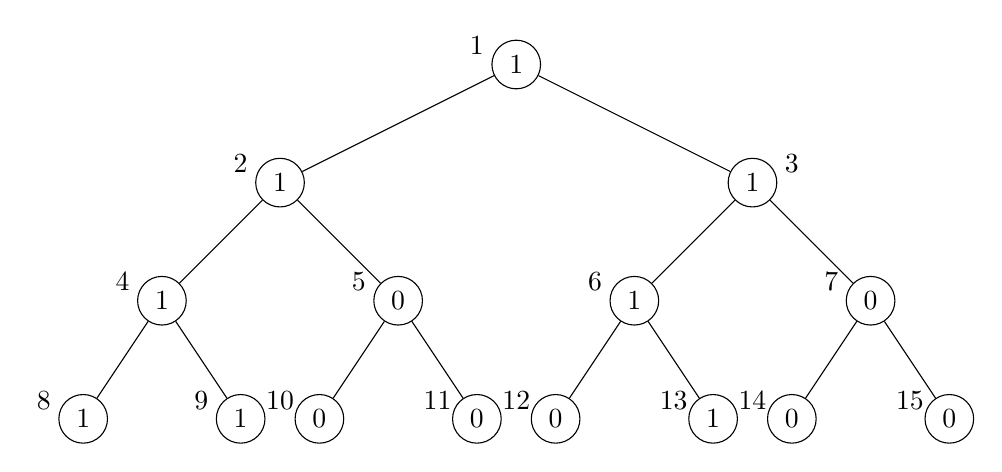
\begin{tikzpicture}[level/.style={sibling distance=60mm/#1}]
        \node [circle,draw] (p){$1$}
          child {node [circle,draw] (a) {$1$}
            child {node [circle,draw] (c) {$1$}
              child {node [circle,draw] (g) {$1$}} 
              child {node [circle,draw] (h) {$1$}}
            }
            child {node [circle,draw] (d) {$0$}
              child {node [circle,draw] (i) {$0$}} 
              child {node [circle,draw] (j) {$0$}}
            }
          }
          child {node [circle,draw] (b) {$1$}
            child {node [circle,draw] (e) {$1$}
              child {node [circle,draw] (k) {$0$}} 
              child {node [circle,draw] (l) {$1$}}
            }
            child {node [circle,draw] (f) {$0$}
              child {node [circle,draw] (m) {$0$}}
              child {node [circle,draw] (n) {$0$}}
          }
        };
        
    \path (p) -- (p) node [left=0.5cm, above] {1};
    \path (a) -- (a) node [left=0.5cm, above] {2};
    \path (b) -- (b) node [right=0.5cm, above] {3};
    \path (c) -- (c) node [left=0.5cm, above] {4};
    \path (d) -- (d) node [left=0.5cm, above] {5};
    \path (e) -- (e) node [left=0.5cm, above] {6};
    \path (f) -- (f) node [left=0.5cm, above] {7};
    \path (g) -- (g) node [left=0.5cm, above] {8};
    \path (h) -- (h) node [left=0.5cm, above] {9};
    \path (i) -- (i) node [left=0.5cm, above] {10};
    \path (j) -- (j) node [left=0.5cm, above] {11};
    \path (k) -- (k) node [left=0.5cm, above] {12};
    \path (l) -- (l) node [left=0.5cm, above] {13};
    \path (m) -- (m) node [left=0.5cm, above] {14};
    \path (n) -- (n) node [left=0.5cm, above] {15};
    \end{tikzpicture}
}
\end{adjustwidth}

%Text for diagram explanation here
\noindent
\\
\begin{text}
    The data structure is represented with a complete binary tree with $2n - 1$ nodes. Each node holds a one bit value of 0 or 1, so the structure takes up $2n - 1$ bits. Let $i$ be the index of a node in the vector, starting from 1. These values are marked outside the node in the diagram. For $n \geq i \geq 2n -1$ (the lowest level in the tree), a value of 1 means that the integer $i - n + 1$ is in the set $S$, while 0 means it's not in $S$. For instance, a value of 1 at index 9 means that $2 \in S$. For all other nodes ($1 \geq i \geq n -1$), a value of 1 means it has a child node whose value is 1, and zero otherwise. Thus, values of 1 in the tree act as paths to the integer values that are present in $S$. The vector representation of this data structure for $n = 8$ and $S = \{1, 2, 6\}$ would be $[1, 1, 1, 1, 0, 1, 0, 1, 1, 0, 0, 0, 1, 0, 0]$.
    \\
\end{text}


\noindent
\textbf{b) Explain how the operations $INSERT(j)$, $DELETE(j)$, and $MAXIMUM$ are executed, and why they take
$O(log(n))$ time in the worst-case.}

\noindent
\begin{text}
    \\\\
    $INSERT(j):$ This function inserts $j \in I_n$ into the data structure. The first step is to change the value at index $j + n - 1$ to 1, if it is not already. Changing the value at this index always takes one step so it's constant time. Let $i = \floor{\frac{i}{2}}$ , which is the index of the parent node of the node representing $j$. We check the value of this parent node; if it is 1, we can return. Else, we set its value to 1 and update $i = \floor{\frac{i}{2}}$. If $i$ is equal to 0, we also return, since we have reached the top. At most this process traverses the entire tree up to the root, making one basic operation on each level. This would take $log_{2}n$ steps, which is the height of the tree. As a whole, $INSERT(j)$ takes $log(n) + 1$ steps in the worse case. Therefore, the worst-case time complexity of this function is $O(log(n))$.\\
    
    \noindent
    $DELETE(j):$ This function deletes a pre-existing $j \in I_n$ from the data structure. We must change the value at index $j + n -1$ (which represents $j$) from 1 to 0. Let $i = \floor{\frac{i}{2}}$, which is the index of the parent node of the node representing $j$. If the node at index $i$ has a child that has a value of 1, stop the operation and the function returns, since we need to keep that path for the other child. If the node has no children with a value of 1, we change the value of the node from 1 to 0 to represent the deletion of a path. We update $i = \floor{\frac{i}{2}}$, and continue these steps until we reach the root node. If we reach the root node, we will have taken at most $2log_{2}(n)$ steps; checking and deleting take 2 steps and we do this for each of the $log n$ levels. Then at most this $DELETE$ takes $2log(n) + 1$ steps and therefore the worst-case time complexity is $O(log(n))$.\\

    \noindent
    $MAXIMUM:$ This function returns the largest number in the set $S$. Let $i = 1$. We start from the node with index $i$ (root node) and check if its value is 1. If it's not, the tree is empty and we return. Else, if its right child's value (value at index $2i + 1$) is 1 we update $i = 2i + 1$ and otherwise we update $i = 2i$. We repeat these steps in a loop and exit the loop when $i \leq 2n - 1$. Then, the last valid node traversed has index $\floor{\frac{i}{2}}$, and we return the value at that index. This operation always takes $log(n) + 1$ steps and therefore the worst-case time complexity is $O(log(n))$.\\
\end{text}

\noindent
\textbf{c) Explain how the operation $MEMBER(j)$ is executed, and why it takes $O(1)$ time in the worst-case.}

\noindent
\begin{text}
    \\\\
    $MEMBER(j):$ This function returns a boolean expression based on if $j$ is in the data structure or not. This simply returns the value of the $n + (j - 1)$'s node, since its value represents the presence of the element in the set $S$. The data structure is set so that the value $n + (j - 1)$ represents the $j$-th node in the $n$-bit vector, thus taking only 1 step to execute, therefore the worst-case time complexity is $O(1)$.
\end{text}
%END Q2

\end{document}